% !TeX spellcheck = en_GB

\chapter{An Adaptive Filter Model of the Cerebellum}
\label{chp:cerebellum}

\vspace{15pt}

\begin{OpeningQuote}
The CNS [Central Nervous System] needs to be understood at four nearly independent levels of description: (1) that at which the nature of a computation is expressed; (2) that at which the algorithms that implement a computation are characterized; (3) that at which an algorithm is committed to particular mechanisms; and (4) that at which the mechanisms are realized in hardware.
In general, the nature of a computation is determined by the problem to be solved, the mechanisms that are used depend upon the available hardware, and the particular algorithms chosen depend on the problem and on the available mechanisms.
\OpeningQuoteSource{David Marr and Tomaso Poggio}{From Understanding Computation to Understanding Neural Circuitry (1976)}
\end{OpeningQuote}

\begin{PriorPublication}
This chapter is, with permission from the publisher, in large parts directly adapted from \citet{stockel2021connecting}.
In turn, this publication is based on work presented at the Cognitive Science Society Conference (\enquote{CogSci}; \cite{stockel2020biologically}) and at the International Conference on Cognitive Modelling (\enquote{ICCM}; \cite{stockel2020connecting}).
\end{PriorPublication}

\begin{Contributions}
The author was responsible for conducting the experiments presented in this chapter, contributing the underlying theoretical work (cf.~previous sections), writing, creating all figures, and conducting literature review.
Terrence C.~Stewart helped with designing the overall network, exploring the parameter space, and writing the paper, in particular the \enquote{Levels of Biological Detail} section.
We heavily edited this section to reduce redundancy with earlier parts of this thesis.
Chris Eliasmith supervised this work and provided important feedback.
The novelty of this work lies in demonstrating that the modelling techniques presented earlier can, together with biological constraints, be used to systematically construct models of complex biological systems.
Our work provides evidence that the Granule-Golgi circuit could generate a temporal basis, a hypothesis that is openly debated in neuroscience.
\end{Contributions}

\clearpage
% !TeX spellcheck = en_GB

Human cognition is ultimately grounded in neurophysiological processes.
As suggested by Marr's \enquote{levels of analysis} \citep{marr1976understanding}, cognitive scientists tend to implement models of cognition at algorithmic and computational levels, without explicitly taking limitations of the underlying neural substrate into account \citep{eliasmith2015marr}.

Depending on the hypothesis that is being explored, ignoring biological detail can be reasonable. Yet, a closer look at biology may help in two complementary ways.
First, we can \emph{validate} hypotheses about cognition by determining whether it is possible to implement a particular algorithm under the constraints of the biological network in question.  
Second, we can \emph{generate} new hypotheses by asking what class of algorithms a certain network could support.

We believe that cognitive modelling must ultimately embrace a combination of top-down and bottom-up modelling to narrow down the vast space of possible cognitive science theories and to direct research attention within that space.
However, a central roadblock to the adaptation of such methods is the availability of modelling tools that make it possible to specify detailed biological constraints (e.g., neural response curves, spike rates, synaptic time-constants, connectivity patters) while still being abstract enough to facilitate the specification of high-level cognitive function.

One approach designed to help bridge this gap is the Neural Engineering Framework (NEF; \cite{eliasmith2003neural}), in conjunction with the related Semantic Pointer Architecture (SPA; \cite{eliasmith2013how}).
Up until recently however, it has been unclear how to incorporate certain biological constraints that are often described in the neuroscience literature into NEF networks.
For example, and despite initial progress in this direction \cite{parisien2008solving}, accounting for Dale's principle with purely excitatory and inhibitory neuron populations, as well as incorporating spatial connectivity constraints, has been relatively challenging with the existing NEF-based software tool, Nengo \cite{bekolay2014nengo}.
Furthermore, there have been no studies on how adding these additional constraints influences the high-level function of NEF networks. In this paper, we attempt to address both issues.

Specifically, we describe recent advances in modeling techniques that partially alleviate the shortcomings of the NEF mentioned above.
We then use these methods to construct a model of eyeblink conditioning in the cerebellum, with a focus on the generation of temporal basis function representations in the recurrent Granule-Golgi circuit.

Building a model of temporal representation in the cerebellum is of particular interest, since it remains unclear how exactly the cerebellum manages to learn and reproduce the precise timings observed in eyeblink conditioning. Furthermore, the mechanisms underlying eyeblink conditioning are potentially exploited by cognitive processes as well. Recent evidence---ranging from studies in functional connectivity, neuronal tracing, clinical pathology, to evolutionary physiology---suggests that the tasks supported by the cerebellum are not restricted to motor control alone. The cerebellum may instead be recruited by various brain regions as a \enquote{co-processor} to support brain functions related to higher-order cognition, such as language-based thinking, working memory, perceptual prediction, and tasks requiring precise timings in general \citep{sullivan2010cognitive,
           buckner2013cerebellum,
		   oreilly2008cerebellum,
           e2014metaanalysis}.

Our experiments suggest that---at least under the constraints we consider---the Granule-Golgi circuit is well-suited to encode temporal information using basis functions. This representation can be used in the context of a spiking neural network to learn delays by modulating synaptic weights in the granular-to-Purkinje projection.
Furthermore, we generate hypotheses as to why various biological parameters (such as the sparse connectivity patterns and the time-constants of the neurotransmitters) are as observed.

The remainder of this paper is structured as follows.
We first review the high-level function we hypothesize could be implemented in the Granule-Golgi circuit, followed by an overview of the eyeblink conditioning task, the particular neurophysiological constraints of the cerebellum, and high-level theories of cerebellar function.
We then discuss five neural network implementations with an increasing amount of biological detail, along with the corresponding extensions to the NEF.
We perform a series of experiments that explore the impact of individual parameters on the performance of the increasingly realistic system.
We extend our model to perform the complete eyeblink conditioning task by incorporating the remaining cerebellar microcircuitry and compare the model behavior to empirical data.
Finally, we provide a quick overview of \enquote{NengoBio,} the open-source addon to Nengo we developed to encode the aforementioned biological constraints.\footnote{See \url{https://github.com/astoeckel/nengo-bio}.}


\clearpage
\setcounter{subsection}{0}
% !TeX spellcheck = en_GB

\section{Background}

In order to explore the consequences of adding biological details to a neural system, we need to choose the desired computation that the neural system should ideally perform.
In machine learning, the simplest artificial neural networks are purely feed-forward, i.e., they possess no backwards-directed or \emph{recurrent} connections. It is well-known that feed-forward neural networks are universal function approximators \citep{hornik1989multilayer}.
That is, given enough neurons, any function $f(x) = y$ can be implemented as a neural network by simply having a single hidden layer of neurons that receives $x$ as an input (via a set of input weights) and produces $y$ as an output (via a set of readout weights).

Neurobiological systems differ from the artificial neural networks mentioned above in two key aspects.
First, they are intrinsically dynamical systems, i.e., input and output are functions over time.
Second, they often include recurrent connections.
As has been shown by \citet{eliasmith2003neural}, adding recurrent connections along with their associated synaptic dynamics allows for the creation of neural networks that approximate any differential equation of the form ${\mathrm{d}\vec m}/{\mathrm{d}t} = {\dot{\vec m}} = f(\vec m, u, t)$, where $f$ is an arbitrary function describing the dynamics, $\vec m$ is the system state, $u$ is an external input, and $t$ is time.
Again, with a sufficient number of neurons and the corresponding connectivity, such differential equations can be approximated to any desired degree of accuracy.
Our primary goal in this paper is to explore how well such computations can be performed in the presence of biological constraints. Once we have established this computational basis, we extend our network to a complete model of the eyeblink conditioning task and compare our simulation results to empirical data.

\subsection{The Legendre Delay Network}

As a benchmark for evaluating the impact of incorporating biological detail into a functional description, we choose the following linear differential equation $\theta\dot{\vec{m}} = \mat{A} \vec m + \mat{B} u$, where
\begin{align}	
    (\mat A)_{ij} &= \begin{cases}
        (2i + 1)(-1) & \text{if }i < j \,,\\
        (2i + 1)(-1)^{i - j + 1} & \text{if } i \geq j \,,
    \end{cases} &
    (\mat B)_i &= (2i + 1)(-1)^i \,.
    \label{eqn:delay_network_lti}
\end{align}
Here, $\vec m$ is a $q$-dimensional vector describing the current state of the linear system, $\mat A$ is a $q \times q$ matrix describing the state evolution, and $\mat B$ is a $q \times 1$ matrix describing how a scalar input $u$ influences the state.
This particular equation has been derived by taking the Padé approximants of the continuous-time delay $F(s)=e^{-\theta s}$ in the Laplace domain.
As such, this differential equation stores a compressed version of the past $\theta$ seconds of its inputs in the state variable $\vec m$ \citet{voelker2018improving}.
That is, given $\vec m$ at any point in time $t$, it is possible to recover an approximate value of $u$ at a previous point in time $\hat u(t - \theta')$ for $0 \leq \theta' \leq \theta$:
\begin{align}
	\hat u(t - \theta')
		&= \sum_{\ell = 0}^{q - 1} m_\ell d_\ell(\theta') \,, & \text{where } d_\ell(\theta') &= \tilde P_\ell \left(\frac{\theta'}{\theta}\right)
		= 
(-1)^\ell \sum_{k = 0}^\ell \binom{\ell}k \binom{\ell + k}k
			\left(-\frac{\theta'}{\theta}\right)^k\,.
	\label{eqn:delay_network_decoder}
\end{align}
The function $\tilde P_\ell$ is the shifted Legendre polynomial of degree $\ell$.

Another way to think of this system is that it encodes the past history of its inputs using a set of \textit{temporal basis functions}. The temporal basis functions that happen to form the representational basis of the above linear system are the Legendre polynomials $\tilde P_\ell$, which have been shown to be optimal for encoding such temporal memory \cite{voelker2018improving}.
Of course, some information is lost in this process of compressing the history of $u$ into $\vec m$. The quality with which past $u$ can be reconstructed from $\vec m$ is controlled by the number of state dimensions $q$, or, more precisely, the ratio of $q$ and $\theta$.
As $q$ increases for a constant $\theta$, more details (i.e., higher frequencies) about the past are represented in $\vec m$.

The neural implementation of this computation is called a \enquote{Legendre Delay Network}~(LDN).
Crucially, arbitrary functions over the time interval $[t - \theta, t]$ can be decoded from the neurons representing the network state $\vec m$, and not just delays. In other words, the LDN forms the filter bank of an adaptive filter, a hypothesized functional description of the Granule-Golgi circuit in the cerebellum \citet{fujita1982adaptive}. The LDN has previously been used to model cognitive timing behavior in humans \citet{jong2019flexible} and is also the core component of a novel machine learning algorithm known as the Legendre Memory Unit~(LMU), which has been shown to outperform LSTMs on several benchmark tasks \citep{voelker2019lmu}.

If we use biologically constrained neural networks to approximate the above linear system, then the actual computation performed by the system, and hence the quality of the time window encoded in $\vec m$, may be different.
We can thus use this system as a benchmark.
In the following, after discussing the cerebellum in more detail, we build various approximations of the LDN using different biological constraints, systematically provide them with inputs, and evaluate their performance in terms of how well the input history can be recovered. Finally, we integrate the LDN into a model of the cerebellum performing the eyeblink conditioning task.
To create the model, we compute optimal input and recurrent connection weights independently for each target population to approximate functional descriptions such as \cref{eqn:delay_network_lti} given biological constraints.
This means we are not modelling the entire developmental process for the cerebellum, but are rather directly creating a model of a mature cerebellum.  For the full eyeblink conditioning task, we then also apply a local biologically plausible learning rule to learn the readout weights.

\subsection{Eyeblink Conditioning}

The cerebellum is well-studied and highly regular in its structure, and there are reasons to believe that the cerebellum does compute something akin to the operation performed by the Legendre Delay Network \citet{fujita1982adaptive}. Behaviourally, the cerebellum is known to be vital for some delay conditioning tasks, such as eyeblink conditioning.

In eyeblink conditioning, a puff of air is directed at the eye (unconditioned stimulus; US), triggering the eyeblink reflex (unconditioned response; UR). The US is paired with a neutral, conditioned stimulus (CS), for example a short tone. The CS precedes the US by a constant time offset $\Delta t$. Over time the subject forms a conditioned response (CR) to the previously neutral CS, maintaining the fixed delay $\Delta t$. In other words, the subject will learn to have its eye closed $\Delta t$ seconds after the tone, even if the puff is absent \citep[cf.][]{heiney2014cerebellardependent}. Experiments indicate that the formation of this conditioned response critically depends on the cerebellum; previously learned CRs are absent once the cerebellum is ablated \citep{mccormick1981engram}.

\subsection{Cerebellar Microcircuitry}

\begin{figure}[t]
	\centering
	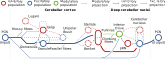
\includegraphics[scale=0.95]{media/chapters/05_cerebellum/cerebellum_anatomy.pdf}
	\caption[Schematic of the cerebellar microcircuit.]{Schematic of the cerebellar microcircuit. Dashed projections and populations are not included in our model. Cerebellar nucleus afferents affect both the excitatory and inhibitory sub-populations.  The main feed-forward pathway is highlighted in bold. \emph{PCN}~$\hat=$~pre-cerebellar neurons/nuclei. \emph{pRN}~$\hat=$~parvicellular Red Nucleus. Data from \citet{ito2010cerebellar,llinas2010olivocerebellar}.}
	\label{fig:cerebellum_anatomy}
\end{figure}

Before we continue to discuss the two prevalent theories on how the cerebellum could learn the conditioned response, it is worthwhile to review the cerebellar microcircuitry depicted in Fig.~\ref{fig:cerebellum_anatomy}.
Afferent nerves from pre-cerebellar (PC) nuclei (brainstem and cerebral cortex carrying sensory signals) project as \enquote{mossy fibers} onto granule cells in the cerebellar cortex.
Cerebellar granule cells are tiny and account for the majority of neurons in the mammalian brain. Thus, very few PC neurons connect onto a very large number of granule cells.

Granule cells also have inter-neurons interspersed amongst them, known as Golgi cells, forming an inhibitory feedback loop with the granule cells. That is, granule cells excite Golgi cells, and Golgi cells inhibit granule cells \citep{ito2010cerebellar}.
Notably, the connections from Golgi and PC cells to granule cells are formed through so called glomeruli. Each granule cells extends to on average four glomeruli and, at each glomerulus, receives input from one PC neuron through a mossy fiber terminal, as well as one or more Golgi cells \citep{palkovits1972quantitative,jakab1988quantitative,chadderton2004integration}.
Furthermore, the connectivity between Golgi and granule cells is spatially constrained, i.e., Golgi cells only connect to granule cells in their vicinity \citep{dangelo2013cerebellar}. The ratio of granule to Golgi cells is about 400:1 \citep{korbo1993total}.

Granule cell axons, the so called \enquote{parallel fibers,} project onto the Purkinje cells, which inhibit neurons in the cerebellar nucleus, and in turn project back onto the brainstem and cerebral cortex \citep{ito2010cerebellar,llinas2010olivocerebellar}. So called \enquote{climbing fibers} project from Inferior Olive neurons in the deep cerebellar nucleus onto Purkinje cells. 
Evidence suggests that activity in the climbing fibers is responsible for modulating the synaptic strength of granule to Purkinje projections. Climbing fiber activity can thus be interpreted as an \enquote{error signal} responsible for driving learning in the cerebellar cortex \citep{ito2010cerebellar}.

\subsection{Hypothesized Mechanisms Supporting Delay Learning}

There is no current consensus on what the exact mechanism is that supports delay learning in the cerebellum.
The classical view is the aforementioned adaptive filter theory \citep{fujita1982adaptive}.
As originally pointed out by \citep{marr1969theory}, the massive divergence (number of post-neurons for a single pre-neuron) and small convergence (number of pre-neurons for a single post-neuron) in the PC to granule projection suggests that granular cells are tuned to specific patterns of activity in the PC neurons.
The adaptive filter theory can be interpreted as extending this idea toward temporal tuning.
Granule cell activity does not only depend on the current PC activities, but on their time-course. Such a temporal tuning could be the result of the recurrent granule-to-granule connections mediated by the inhibitory Golgi cells.
If this temporal tuning is diverse enough, i.e., granule cells are sensitive to different time-courses, this will form a suitable temporal basis from which arbitrary delays can be decoded.
Learning a specific decoding is driven by the climbing fiber error signal, modulating the synaptic weights between the granule and the Purkinje cells.
As mentioned above, this is similar in principle to the Legendre Delay Network.

A more recent theory is that responses observed in tasks such as eyeblink conditioning inherently rely on intrinsic properties of the Purkinje cells.
In other words, temporal properties of the granule cells play a lesser role.
Instead, climbing fiber input triggers processes within the Purkinje cell and their dendritic structures that are responsible for the formation of a delayed output.
Indeed, \citet{johansson2014memory} find that bypassing the granule cells and directly injecting signals into the parallel fibers still evokes a previously learned delayed response from the cerebellum, albeit a weaker one.

We think that these two theories are not inherently contradictory. Both temporal tuning of the granular cells and intrinsic temporal properties of the Purkinje cells could play a role in delay learning.
The findings we present in this paper provide a strong argument that the biology of the Granule-Golgi circuit is at least well suited for implementing some kind of temporal basis function generation, and as such confirms the results of previous studies  \citep[cf.][]{dean2010cerebellar,rossert2015edge}.
Still, our work only takes a fraction of the available data on cerebellar neurophysiology into account and as such should not be seen as strong evidence for or against one of the two proposed mechanisms.
Instead, we are interested in describing methods for adding biological constraints while determining their consequences for higher-level function.


\clearpage
\setcounter{subsection}{1}
% !TeX spellcheck = en_GB

\section{Levels of Biological Detail}

To demonstrate our approach of adding biological detail, we first focus on a model of temporal basis function generation in the Granule-Golgi circuit discussed above.
We present five models of increasing complexity---the first model is merely an abstract implementation of \cref{eqn:delay_network_lti}, the final model respects spatial sparsity, convergence, tuning curves, and, to a degree, neurotransmitter constraints.
All models are depicted in Fig.~\ref{fig:network_types}.
In all cases, the scalar input $u$ is received from one hundred spiking Leaky Integrate-and-Fire (LIF) neurons with randomly chosen tuning curves, representing input provided by the PCN (see Model B for details).

\paragraph{Model A: \enquote{Direct} Implementation} 
For this model, we directly solve the differential equation in \cref{eqn:delay_network_lti} by integration.
That is, we have a single layer of \enquote{neurons} that are pure integrators (i.e., no non-linearity). The matrix $\mat{A}$ describes the recurrent connection weights, and $\mat{B}$ the input connection weights.
This model does not distinguish between the granule and Golgi cells, and does not include details such as individual neurons or spikes.
Instead, it focuses on the high-level theory of what the system is computing.

\paragraph{Model B: Single Population}
We replace the integrators with a single layer of 200 spiking Leaky Integrate-and-Fire (LIF) neurons.
These neurons form a distributed representation of $\vec{m}$ using a population code.
Each neuron $i$ is parametrized by a randomly chosen preferred stimulus vector $\vec{e}_i$ (for \textit{encoder}), gain $\alpha_i$ and bias current $J^\mathrm{bias}_i$, resulting in a desired response (i.e., tuning curve) for each neuron:
\begin{align}
    a_i(\vec m) = G[J_i(\vec m)] = G[\alpha_i (\vec{e}_i \cdot \vec{m} ) + J^\mathrm{bias}_i] \,,
    \label{eqn:lif_tuning_curve}
\end{align}
where $G$ the is neural response curve of the LIF neuron model.
The parameters $\alpha$ and $J_\mathrm{bias}$ are randomly chosen from a distribution that ensures a maximum firing rate of \SIrange{50}{100}{\hertz}, consistent with biological recordings of granule cells \cite{chadderton2004integration}.
We then use least-squares to solve for optimal input and recurrent connection weights that result in these desired tuning curves while implementing the equivalent calculation as in Model A.
Importantly, when solving for the recurrent connection weights, we also take into account the synaptic filter, which we model here as a decaying exponential (i.e., a low-pass).
This is the standard process in the NEF \cite{eliasmith2003neural}.

\paragraph{Model C: Inter-neurons}
As a next step, we separate the single layer of neurons into two populations corresponding to the Golgi and granule cells, reflecting the actual biology of the cerebellum (see above). This introduces two synaptic filters which need to be taken into account when solving for the connection weights that best approximate \cref{eqn:delay_network_lti}.
Furthermore, to at least approximate the fact that there are far fewer Golgi cells than granule cells, we use 20 Golgi cells and 200 granule cells.

\paragraph{Model D: Inhibition and Excitation}
So far, we have not accounted for Dale's principle, i.e., Golgi cells being purely inhibitory, and granule cells being purely excitatory.
We handle this by switching to the non-negative least-squares problem described in \citet{stoeckel2021passive}. For each post-neuron $i$ we minimize
\begin{align*}
    \min_{\vec w_i^+, \vec w_i^-} \sum_{k = 1}^N \big( \vec w_i^+ \cdot \vec a^+_k - \vec w_i^- \cdot \vec a^-_k - J_i(\vec m_k) \big)^2 \; \text{ w.r.t.} \; \vec w_i^+, \vec w_i^- \geq 0 \,,
\end{align*}
where $\vec a^+_k$, $\vec a^-_k$ are the excitatory and inhibitory pre-activities for sample $k$, $\vec w^+$, $\vec w^-$ are the connection weights for excitatory and inhibitory pre-neurons, and $J_i(\vec m_k)$ is the current required to represent the desired value $\vec m_k$ as defined in \cref{eqn:lif_tuning_curve}.

\begin{figure}[t]
    \centering
    \includegraphics{media/chapters/05_cerebellum/spatial_constraints.pdf}
    \caption[Spatial connectivity constraints.]{Spatial connectivity constraints. \textbf{(A)} Normalized connection probabilities $p_{ij}$ for $\sigma=0.25$. \textbf{(B)} Spatial organisation of the Golgi and granule cells. The background depicts the cumulative density of the Golgi to granule connection probability for a virtual Granule cell at each location (same colours as in \textbf{A}).}
    \label{fig:spatial_constraints}
\end{figure}

\paragraph{Model E: Sparse connectivity and activity}
For this model, we add in realistic constraints on how connected the neurons are.
The previous models used all-to-all connections, whereas for this model, we only allow a subset of those connections to be non-zero.
This applies to both the input to the Granule-Golgi system and for the recurrent connections within the granule cells.  
In particular, we account for the granule cell convergence numbers by randomly selecting five PCN and five Golgi cells as pre-neurons---this number is slightly larger than the number reported above, since, as we discuss below, the number of pre-neurons places a strict upper limit on the connectivity. Given this extremely sparse connectivity, we increase the number of neurons in the simulation to 10\,000 granule and one hundred Golgi cells, which is closer to the ratio observed in nature.

To account for spatially imposed connectivity constraints, we assign a location $\vec x$ in $[-1, 1]^2$ to each neuron. The probability $p_{ij}$ of a post-neuron $i$ to receive a connection from a pre-neuron $j$ is proportional to $\exp \left(- \| \vec x_i - \vec x_j \|^2 / \sigma^{2} \right)$ (Fig.~\ref{fig:spatial_constraints}).

Finally, the input representation in the PC neurons was made more temporally sparse by adjusting the gain and bias parameters in \cref{eqn:lif_tuning_curve}.
Data reported by \citet{chadderton2004integration} indicate that granule cell excitatory event rates---which are driven by PCN activity---drop from an average of \SI{40}{\per\second} with a stimulus being present to only \SI{8.5}{\per\second} when there is no stimulus.
We adjusted the PCN tuning curves to match these statistics in the final network.


\clearpage
\setcounter{subsection}{2}
% !TeX spellcheck = en_GB

\section{Experiments and Results}


\begin{figure}[t]
	\centering
	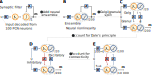
\includegraphics{media/chapter_cerebellum/network_types.pdf}
%	\begin{subfigure}{1.4in}%
%		\centering%
%		\includegraphics[scale=0.95]{media/network_types_a.pdf}%
%		\phantomcaption%
%		\label{fig:network_types_a}%
%	\end{subfigure}%
%	\begin{subfigure}{1.4in}%
%		\centering%
%		\includegraphics[scale=0.95]{media/network_types_b.pdf}%
%		\phantomcaption%
%		\label{fig:network_types_b}%
%	\end{subfigure}%
%	\begin{subfigure}{1.4in}%
%		\centering%
%		\includegraphics[scale=0.95]{media/network_types_c.pdf}%
%		\phantomcaption%
%		\label{fig:network_types_c}%
%	\end{subfigure}%
%	\begin{subfigure}{1.4in}%
%		\centering%
%		\includegraphics[scale=0.95]{media/network_types_d.pdf}%
%		\phantomcaption%
%		\label{fig:network_types_d}%
%	\end{subfigure}%
%	\begin{subfigure}{1.4in}%
%		\centering%
%		\includegraphics[scale=0.95]{media/network_types_e.pdf}%
%		\phantomcaption%
%		\label{fig:network_types_e}%
%	\end{subfigure}%
	\caption[Network types used in the cerebellum experiments.]{Network types used in our experiments. \textbf{(A)} \enquote{Direct} implementation with an optimal integrator. \textbf{(B)} Using the synaptic filter of a single population of spiking neurons for temporal integration. \textbf{(C)} Inter-neuron population in the recurrent path. \textbf{(D)} Same as \textbf{C}, but accounting for Dale's principle. \textbf{(E)} Same as \textbf{D}, but with more detailed biological constraints (see text).}
	\label{fig:network_types}
\end{figure}

\begin{figure}[t]
	\centering
	\includegraphics{media/chapter_cerebellum/2d_sweeps.pdf}
	\caption[Delayed signal reconstruction errors in the Cerebellum model.]{Delayed signal reconstruction error for different types of input signals, delays, and network types. All error values are expressed as RMSE divided by the average RMS of the input signal over ten trials. Columns correspond to the network types in Fig.~\ref{fig:network_types}. \emph{Top row:} Reconstruction error for rectangle pulse signals of varying width. \emph{Bottom row:} Reconstruction error for a band-limited white noise input signal with varying band-limit.}
	\label{fig:basic_results}
\end{figure}

\begin{figure}
	\centering
    \includegraphics{media/chapter_cerebellum/delay_example.pdf}
	\caption[Examples showing the delayed input signals decoded form the granule layer in the detailed model.]{Examples showing the delayed input signals decoded form the granule layer in the detailed model (Fig.~\ref{fig:network_types_e}). \emph{Top row:} Input signal (rectangle pulses in \textbf{A}, white noise in \textbf{B}). \emph{Middle row:} Spike raster for 40 randomly selected granule cells. \emph{Bottom row:} Delays decoded from one thousand randomly selected granule cells. Dotted lines correspond to an optimal delay.}
	\label{fig:sample_run}
\end{figure}

In the following, we discuss three experiments. First, we analyze the temporal representations produced by each of the increasingly constrained models described above. Second, we systematically vary model parameters to gain a better understanding of why certain parameters are as observed. Third, we extend our model to incorporate the remaining components of the cerebellar microcircuit discussed above, resulting in a complete model of eyeblink conditioning.

\subsection{Influence of biological constraints on temporal representations}

To evaluate the effects of these biological details, we systematically generate two different types of input $u(t)$, feed those into the network and record the resulting activity.
In particular, we present results with a periodic pulse input of varying pulse width $t_\mathrm{on}$ and band-limited white noise of varying bandwidth $B$. These are meant to depict typical sorts of inputs that may arise in experimental situations (pulses) and more real-world situations (band-limited white noise).
We then determine how accurately the past history of $u$ over the window $\theta$ can be recovered from the resulting network activity via optimal linear readout weights. We use $\theta = \SI{0.4}{\second}$ in all simulations; each individual experiment simulates the network for $T = \SI{10}{\second}$.
The error is the RMSE of the reconstruction divided by the RMS power of the input itself (normalized RMSE, or NRMSE).

The overall results for all five models are shown in Fig.~\ref{fig:basic_results}.
This shows the average reconstruction error for varying inputs (horizontal axis) and for varying time delays (vertical axis) over ten trials.
An example run of Model E (the model with the most biological detail) is shown in Fig.~\ref{fig:sample_run}.
The different decoded output lines (bottom) are all based on the same neural activity (middle), but with different readout weights.
These approximate the input value $u$ with various time delays over the entire time window, from the immediate input right now ($\theta'/\theta=0$) to $\theta$ seconds ago ($\theta'/\theta=1$).  

As can be seen in Fig.~\ref{fig:basic_results}, the network successfully functions as a method for encoding the temporal pattern of input data over the desired window of time $\theta$.
Adding more biological detail decreases the accuracy with which the system approximates \cref{eqn:delay_network_lti}, but most of the information is still encoded.
The pulse input (Fig.~\ref{fig:sample_run}A) shows that the reconstruction is a smoother version of the input; the system is not good at representing sudden changes, and this is the main source of noise in the reconstruction.  This is as expected from using smooth Legendre polynomials as temporal basis functions. Furthermore, we note that there is a peak in accuracy when decoding data from $\theta' = \SI{60}{\milli\second}$ in the past ($\theta'/\theta=0.15$), and this peak is more pronounced as more biological detail is added. This corresponds to the neurotransmitter time-constant $\tau = \SI{60}{\milli\second}$ we use for all connections, and which is based on a first-order low-pass fit to the NMDA Granule-Golgi dynamics reported in \citet{dieudonne1998submillisecond}. Note that the reported time-constants of other connections in the system are significantly shorter \cite{kanichay2008synaptic}. Techniques described by \cite{voelker2018improving} could be used to compute the connections weights for these heterogeneous time-constants. Yet, for the sake of simplicity, here we assume homogeneous time-constants.

\subsection{Parameter exploration}

\begin{figure}[t]%
%	\begin{subfigure}{0.26\textwidth}%
%		\centering%
%%		\includegraphics[trim=0.2cm 0.3cm 0.25cm 0.25cm,clip,scale=0.95]{media/sweep_tau.pdf}%
%		\phantomcaption%
%		\label{fig:sweep_tau}%
%	\end{subfigure}%
%	\begin{subfigure}{0.21\textwidth}%
%		\centering%
%%		\includegraphics[trim=0.25cm 0.3cm 0.25cm 0.16cm,clip,scale=0.95]{media/sweep_n_pcn_granule_convergence.pdf}%
%		\phantomcaption%
%		\label{fig:sweep_pcn_gr_conv}%
%	\end{subfigure}%
%	\begin{subfigure}{0.21\textwidth}%
%		\centering%
%%		\includegraphics[trim=0.25cm 0.3cm 0.25cm 0.125cm,clip,scale=0.95]{media/sweep_n_golgi_granule_convergence.pdf}%
%		\phantomcaption%
%		\label{fig:sweep_go_gr_conv}%
%	\end{subfigure}%
%	\begin{subfigure}{0.32\textwidth}%
%		\centering%
%%		\includegraphics[trim=0.25cm 0.3cm 0.25cm 0.1cm,clip,scale=0.95]{media/desired_vs_measured_pcn_convergence.pdf}
%		\phantomcaption%
%		\label{fig:convergence}%
%	\end{subfigure}
	\centering
	\includegraphics{media/chapter_cerebellum/parameter_sweeps.pdf}%
	\includegraphics{media/chapter_cerebellum/convergence_histogram.pdf}
	\caption[Cerebellum model parameter exploration.]{Parameter exploration. \textbf{(A-C)} Effects of varying parameters on the delay reconstruction error (arrows indicate default parameters). The box plots show the median, lower and upper quartile of all the data depicted as a contour plot in Fig.~\ref{fig:basic_results}; whiskers are the min/max. The total number of data-points in each bar plot is $n = 441$. \textbf{(D)} Histograms showing the frequency of measured PCN to granule convergences.}
	\label{fig:param_sweeps}
\end{figure}

Notably, we can use our model to determine what the accuracy would be like if we changed individual parameters, such as the aforementioned synaptic time-constant.
This is shown in Fig.~\ref{fig:sweep_tau}.
Interestingly, the performance of the system is best for a filter time-constant of \SI{50}{\milli\second}, which is closed to the value we used based on measured Granule-Golgi dynamics.

As discussed above, a striking feature of the cerebellar microcircuitry is the low granule cell convergence. One possible hypothesis is that these numbers are a trade-off between minimizing connectivity and the overall performance of the resulting system.
In our model, we can test this hypothesis by systematically varying the number of pre-neurons the solver has access to. Results are shown in Figs.~\ref{fig:param_sweeps}B and C.

For the PCN to Granule convergence (Fig.~\ref{fig:param_sweeps}B) the performance of the system does improve with larger limits, yet plateaus at still relatively small convergence numbers.
Importantly, as mentioned above, the specified desired convergence solely controls the number of \emph{potential} pre-neurons.
Since the neural weight solver may still set a weight to zero, these convergence numbers are strict upper limits.
Measuring the actual convergence in the PCN to granule connections (Fig.~\ref{fig:param_sweeps}D), we see a peak at one to three PC neurons connecting to each granule cell, and this peak is only weakly affected by the desired convergence number.
Importantly, in nature, PC neurons connect to on average four granule cells (see \cite{palkovits1972quantitative}, for the complete statistics), whereas we only measure an average convergence of two in our model (for a desired convergence of five).
We can match the observed average in our model by increasing the desired convergence to 13. This slightly increases the performance of the system and coincides with the optimal desired convergence depicted in Fig.~\ref{fig:param_sweeps}B.
Nevertheless, since the gain in performance is relatively small, we decided not to alter the desired convergence in our model setup.

Fig.~\ref{fig:param_sweeps}C indicates that the performance of the system improves up to a desired Golgi to granule convergence number of thirteen, with a measured average convergence of $4.8$ in the final network.
This is a little higher than what is commonly assumed in the neuroscience literature, although, notably, there is some uncertainty regarding this number.
The original study by \citet{jakab1988quantitative} on the physiology of individual glomeruli (the sites receiving Golgi cell axons and granule cell dendrites; cf.~Fig.~\ref{fig:cerebellum_anatomy}) counts up to 145 Golgi axon synapses in one glomerulus.
However, it is unclear whether these synapses originate from a single or different Golgi cells.
Most researchers assume at most one Golgi cell connecting to each glomerulus, and, as explained above, each granule cell in turn connecting to on average of four glomeruli \cite{palkovits1972quantitative}.
Our model predicts that if the Granule-Golgi circuit were to optimally generate a temporal basis, then multiple Golgi cells should sometimes connect to the same glomerulus.

\subsection{Extension Toward a Model of Eyeblink Conditioning}

Given the above model for the Golgi and granule cells, we can now introduce learning into the model to test the behavior of the system in an eyeblink conditioning task.
As discussed above, the error signal $\varepsilon(t)$ originates from the Inferior Olive (IO).
This signal needs to represent the difference between the conditioned response (CR; i.e., what the model has learned so far), and the unconditioned response (UR; i.e., the motor response produced by the innate eyeblink reflex).
These are the two inputs to the IO shown in \Cref{fig:cerebellum_anatomy}.
The CR is the inhibitory input from the Cerebellar Nucleus (CN), and the UR is the excitatory input from the PCN.  

To create a neural version of this, we use a similar approach as described in the second version of the Granule-Golgi circuit.
That is, we train a single-hidden-layer neural network for each of the IO, CN, and pRN using least-squares, and then combine the $\mat{D}$ and $\mat{E}$ matrices to form connection weights.
This is a standard technique when building NEF models.

To adjust the connection weights between the Granule cells and the Purkinje cells, we use the Prescribed Error Sensitivity (PES) rule defined by \citet{macneil2011finetuning}, a biologically plausible variant of the classic delta learning rule.
Let $w^{\mathrm{Gr}\to\mathrm{Pu}}_{ij}$ be the connection weight between the $j$th granule cell and the $i$th Purkinje cell, $\eta$ a learning rate parameter, $a^\mathrm{Gr}_j(t)$ the $j$th post-synaptic granule cell activity filtered by a low-pass filter with time-constant $\tau_\mathrm{learn}$, and $e^\mathrm{Pu}_i \in \{-1, 1\}$ the encoder of the $i$th Purkinje cell, determining whether this cell is an on- or off-neuron.
The delta learning rule is given as
\begin{align}
	\frac{d}{dt} w^{\mathrm{Gr}\to\mathrm{Pu}}_{ij}(t) &= -\eta \varepsilon(t) e^\mathrm{Pu}_i a^\mathrm{Gr}_j(t) \,.
	\label{eqn:delta}
\end{align}
This learning rule can be derived from gradient descent in a single-layer network.
For a small enough $\eta$, the weights are guaranteed to converge to the least-squares solution used in the previous experiments.
The PES rule is given by rewriting \cref{eqn:delta} in terms of local weights and activities
\begin{align*}
	\frac{d}{dt} w^{\mathrm{Gr}\to\mathrm{Pu}}_{ij}(t) &= -\eta \sum_{k} w^{\mathrm{IO}\to\mathrm{Pu}}_{ik} a^\mathrm{IO}_k(t) a^\mathrm{Gr}_j(t) \,,
\end{align*}
where $a^\mathrm{IO}_k(t)$ is the activity of the $k$th IO cell and $w^{\mathrm{IO}\to\mathrm{Pu}}_{ik}$ are the synaptic weights between the $k$th IO cell and the $i$th Purkinje cell. These weights are the product of the Purkinje cell encoder $e_i^\mathrm{Pu}$ and a decoding vector $\vec d_k^\mathrm{IO}$ that linearly decodes the error signal $\varepsilon(t)$ from IO cell activity.

\begin{figure}[t]
	\centering%
%	\includegraphics[]{media/results_panel.pdf}\\[-0.15cm]
	\caption[Model and experimental data for the eyeblink conditioning task.]{Model and experimental data for the eyeblink conditioning task. \textbf{(A, B)} Maximum CR triggered eyelid closure over 500 trials for six random instances of the model/experimental animals. Gray dots correspond to the eyelid closure at the time of the US. Black line is the moving average over 11 trials. Blue dotted lines correspond to an experimental day (100 trials). \textbf{(C, D)} Eyelid closure trajectory averaged over one experimental day and all six models/animals. \textbf{(E)} Eyelid velocity signal decoded at the Purkinje cells compared to the reflex-triggered velocity signal. Data for \textbf{(B, D)} adapted from \protect\citet{heiney2014cerebellardependent}.}
	\label{fig:result-basic}
\end{figure}

\Cref{fig:result-basic} shows the behaviour of a typical run of the detailed version of our model performing the eyeblink conditioning task over 500 trials.
The \enquote{tone} (CS) is modeled as a rectangle pulse with $t_\mathrm{on} = \SI{100}{\milli\second}$.
The \enquote{puff} (US) occurs \SI{250}{\milli\second} after the CS onset.
The model learns to have the eye closed when the puff occurs. Notably, individual instances of the network show slight differences in learning speed, just as individual experimental animals do.

While our model reproduces key features of eyeblink conditioning, its behavior differs from the experimental data in some aspects.
Foremost, the model does not reproduce the increase in learning speed over time; to the contrary, learning slows down as the model converges to the optimal set of parameters.
Furthermore, our model shows far less inter-trial variance compared to experimental animals.
We think that the reasons for this are twofold.
First, the $10\,000$ granule cells used in our experiments provide an on average very stable temporal basis from which we can decode the motor control signal.
Second, we do not model external systems that might interfere with the cerebellar motor commands, such as signals originating from motor cortex, or the physics of the eyelid itself.
Since these processes may be a significant source of inter-trial variance, it is not unsurprising that our model produces a relatively noise-free output.
Still, more research in these areas will be required in the future.

Most parameters were set based on biological data; the synaptic time-constant $\tau = \SI{5}{\milli\second}$ except in the Granule-Golgi microcircuit, as described above.
The only free parameters are the learning rate $\eta=140\times 10^{-6}$, $\tau_\mathrm{pRN} = \SI{100}{\milli\second}$ for the connections involving the pRN, and $\tau_\mathrm{learn} = \SI{60}{\milli\second}$ for filtering the granule cell activity in the learning rule.
The learning rate was adjusted to match the number of trials typically needed for mice to learn the task ($\sim 300$ trials).
Velocity commands smaller than $v_\mathrm{th} = \SI{2}{\milli\metre\per\second}$ are counted as zero.

The low-pass filter $\tau_\mathrm{learn}$ on the learning connection is required to reproduce the observation that the animal will close the eye slightly \emph{before} the puff occurs as learning progresses.
Without the additional filter the system learns to close the eye soon \emph{after} the puff.  This is because it is trying to do exactly what we have asked it to: learn to re-create the same motor pattern as is produced by the unconditioned reflex.  But, the unconditioned reflex closes the eye \emph{after} the puff happens, which is too late.  However, by slowing the passage of information from the Cerebellar Nucleus back to the Inferior Olive (where the comparison between the UR and CR occurs), we are effectively comparing the reflex at one point in time to the generated output from the cerebellum at an \emph{earlier} point in time.  This allows the new learned reflex to occur slightly earlier than the unconditioned response, and thus the eye closes before the air puff.  We note that this is a situation where adding biological detail (the synaptic filtering) improves the performance of the model.  If the model were to learn to \textit{exactly} reproduce the UR given the CS, then the eyeblink would occur \textit{after} the puff of air, which would be a less useful response.


\clearpage
\setcounter{subsection}{3}
% !TeX spellcheck = en_GB

\section{Discussion}

We mapped a high-level, mathematical function onto a brain microcircuit while incorporating biological constraints.
Although we were not able to precisely fit the desired Legendre system onto the most detailed Granule-Golgi circuit, the resulting system implicitly produces a good temporal representation, and the quality of this representation critically depends on trying to implement the Legendre system.

The key difference of our approach to existing models of the Granule-Golgi circuit (such as \cite{rossert2015edge}) is that our modelling techniques are more general with respect to the high-level function that is being mapped onto the underlying circuit.
Instead of relying on random connectivity, we specify the high-level function we would like the system to perform.

\subsubsection{Predictions}
We demonstrated that measurements from our model can be used to generate hypotheses about the kind of electrophysiological data we would expect to find, if this function was indeed realised in the brain.
Having access to low-level biological parameters \emph{in silico} furthermore facilitates the exploration of physiological changes that are difficult to achieve experimentally \emph{in vivo}.
As discussed above with respect to the synaptic time-constants and convergence numbers, this allows us to investigate why certain parameters are as observed.

Importantly, our results indicate that the Granule-Golgi circuit could in principle implement a temporal basis function representation.
However, as we discussed above, this is under the condition that the Granule cell response curves are diversified by some mechanism not directly captured by our model.
Without diverse granule tuning curves the expressiveness of the generated temporal representation is reduced, although not fully unusable.
We furthermore predicted that the Granule-Golgi circuit would be better suited for temporal basis function generation if more than one Golgi cell would sometimes connect to a glomerulus.

\subsubsection{Future work}
While our model of eyeblink conditioning is concerned with a relatively low-level task, the techniques presented here for mapping function onto brain microcircuits are applicable to models of higher-level cognitive function as well, beyond what was already possible with the \NEF and Nengo.
In particular, it would be interesting to see whether our model of the Granule-Golgi circuit in conjunction with the Purkinje cell's plasticity could serve as a supervised learner for timings in cognitive and perceptual tasks, as suggested by various studies \citep{oreilly2008cerebellum,e2014metaanalysis,sanger2020expansion}.

Future work should focus on incorporating additional biological detail into the model (such as separate biological time-constants for all synapses); specifically, it would be interesting to extend the rigour applied to the Granule-Golgi circuit to the remaining portions of the cerebellar microcircuit.
Furthermore, it would be interesting to find potential mechanisms for the diversification of the Granule cell tuning curves and to gain a better understanding of why the Legendre system cannot be mapped exactly onto the detailed Granule-Golgi circuit.
